% !TEX encoding = UTF-8 Unicode
% -*- coding: UTF-8; -*-
% vim: set fenc=utf-8

\section{Databázové schéma}\label{sec:databázovéSchéma}

Jelikož jsem se rozhodl použít \gls{NoSQL} databázi, nemám jak pevně definovat databázové schéma jako v obvyklé relační databázi.
Konzistenci a validitu ukládaných dat musí zajistit sama aplikace a to jak při čtení, tak i při zápisu dat.

Z tohoto důvodu jsem se rozhodl použít \gls{ODM} nástroj Mongoose, který umožňuje v rámci aplikace definovat struktury jednotlivých dokumentů pro MongoDB a jejich validitu kontroluje před každým uložením.
Schéma na obrázku~\ref{fig:DB_model} není databázovým schématem v pravém slova smyslu, ale jedná se o schéma definované za pomoci právě \gls{ODM} Mongoose.

\begin{figure}[ht]
    \centering
    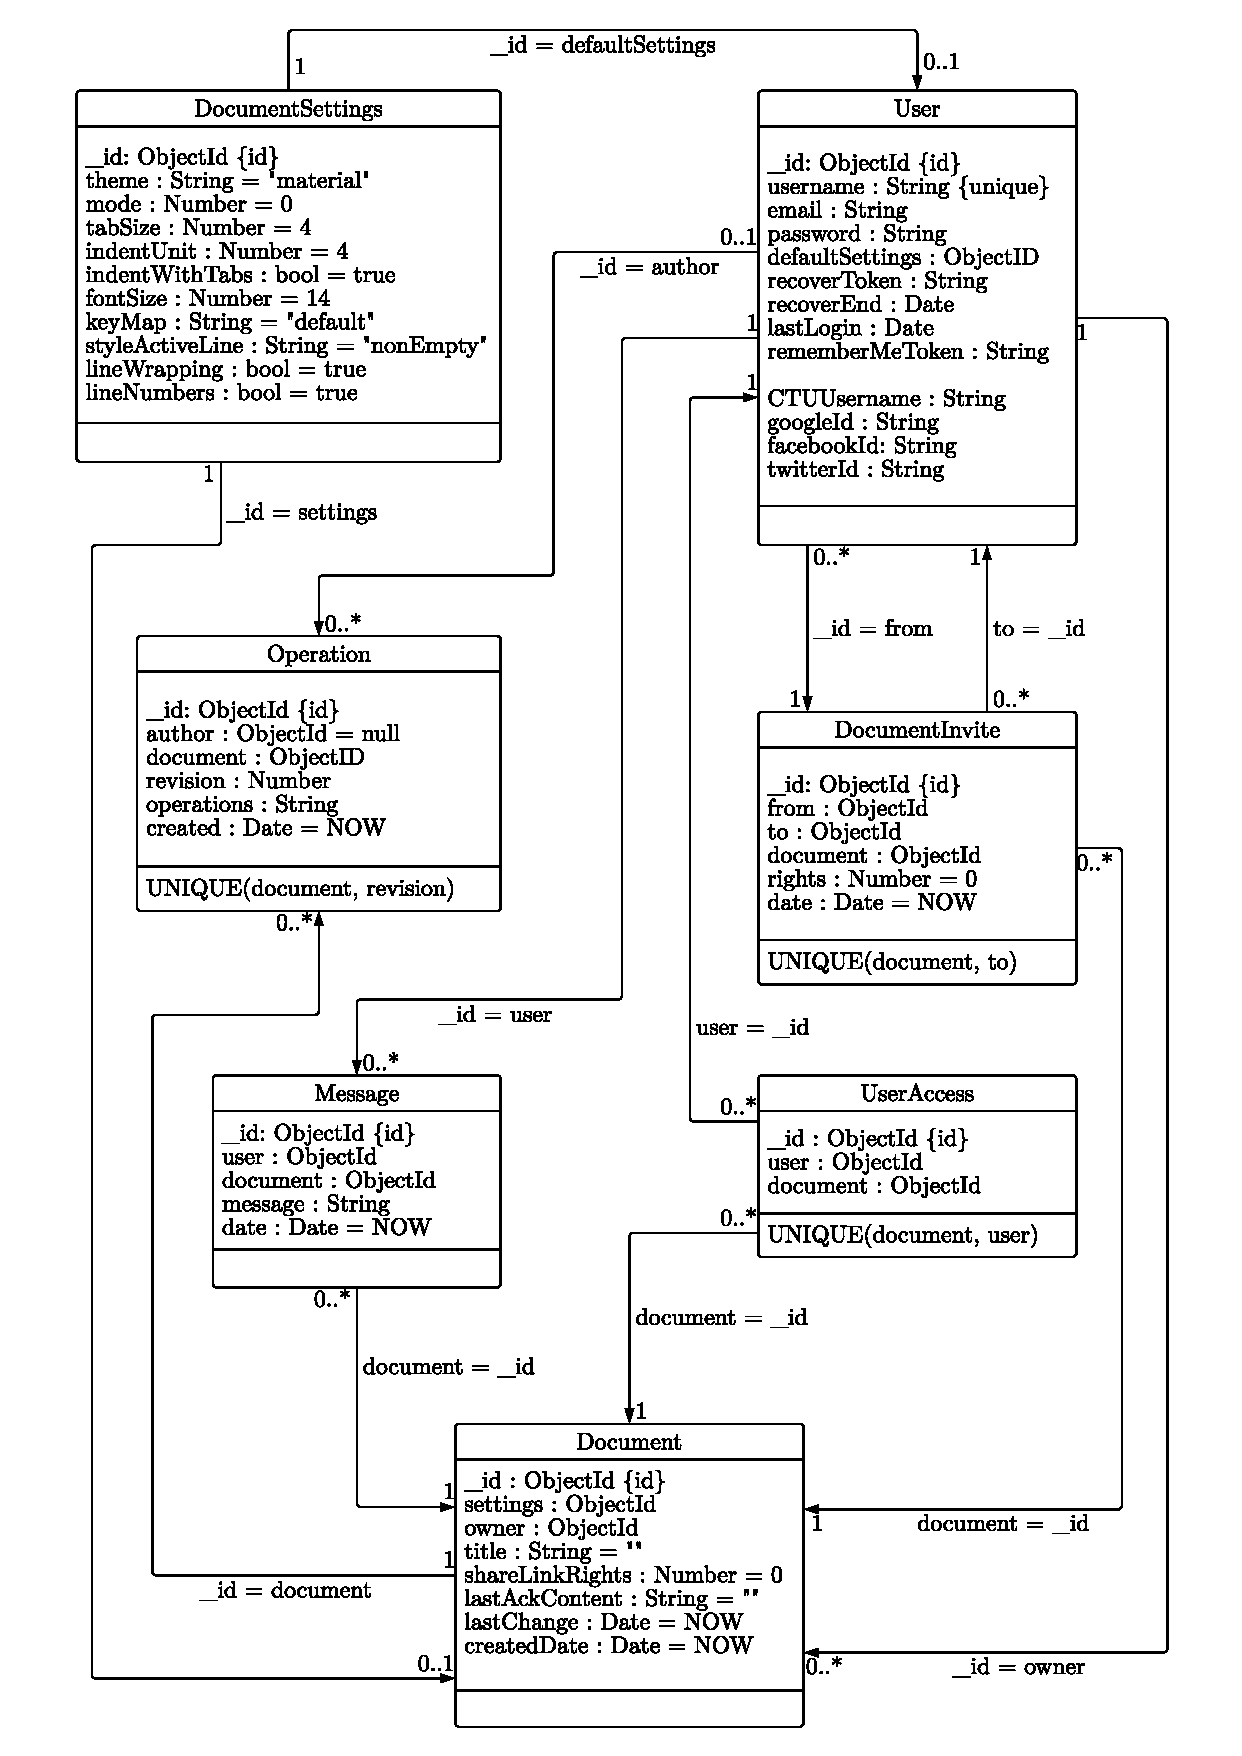
\includegraphics[width=\textwidth]{partials/navrh/DB_model.pdf}
    \caption{Databázové schéma v rámci ODM Mongoose}\label{fig:DB_model}
\end{figure}

Jednotlivé entity schématu přímo reflektují entity z doménového modelu uvedeného v sekci~\ref{sec:domenovyModel}.
Přibyly pouze implementační detaily a atributy jednotlivých relací mezi entitami.
Také se změnily názvy entit a jejich atributů z českého do anglického jazyka, aby lepé reflektovali samotný kód aplikace.

% TODO: upravit cestu podle finální přílohy
Kompletní definice schématu lze nalézt spolu s ostatními zdrojovými kódy na přeloženém CD ve složce \texttt{/app/src/model}.
Na definici lze i mimo jiné pozorovat validační pravidla pro jednotlivé atributy, jako jsou například číselné rozsahy, maximální délky atd.
